\documentclass[10pt,english]{article}

\usepackage{fourier}

\usepackage[]{graphicx}
\usepackage[]{color}
\usepackage{xcolor}
\usepackage{alltt}
\usepackage{listings}
\usepackage[T1]{fontenc}
\usepackage[utf8]{inputenc}
\setlength{\parskip}{\smallskipamount}
\setlength{\parindent}{5ex}
\usepackage{indentfirst}
\usepackage{listings}
\usepackage{setspace}
\usepackage{hyperref}
\hypersetup{
    colorlinks=true,
    linkcolor=auburn,
    filecolor=magenta,      
    urlcolor=blue, urlsize=2em
}

% Set page margins
\usepackage[top=100pt,bottom=100pt,left=68pt,right=66pt]{geometry}

% Package used for placeholder text
\usepackage{lipsum}

% Prevents LaTeX from filling out a page to the bottom
\raggedbottom


\usepackage{fancyhdr}
\fancyhf{} 
\fancyfoot[C]{\thepage}
\renewcommand{\headrulewidth}{0pt} 
\pagestyle{fancy}

\usepackage{titlesec}
\titleformat{\chapter}
   {\normalfont\LARGE\bfseries}{\thechapter.}{1em}{}
\titlespacing{\chapter}{0pt}{50pt}{2\baselineskip}

\usepackage{float}
\usepackage{verbatim}
\floatstyle{plaintop}
\restylefloat{table}

\usepackage[tableposition=top]{caption}


\definecolor{light-gray}{gray}{0.95}

\renewcommand{\contentsname}{Índice}

\begin{document}


\begin{titlepage}
	\clearpage\thispagestyle{empty}
	\centering
	\vspace{2cm}

	
	{\Large  Tecnologias e Programação Web \par}
	\vspace{0.5cm}
	{\small Professor: \\
	Hélder Zagalo\par}
	\vspace{4cm}
	{\Huge \textbf{Aplicação \textit{Web} com \textit{DRF} e \textit{Angular}}} \\
	\vspace{1cm}
	\vspace{4cm}
	{\normalsize Hugo Paiva, 93195 \\ 
	             Daniel Gomes, 93015 \\
	             Pedro Bastos, 93150
	   \par}
	\vspace{2cm}

    
\includegraphics[scale=0.20]{logo_ua.png}
    
    \vspace{2cm}
    
	{\normalsize DETI \\ 
		Universidade de Aveiro \par}
		
	{\normalsize 20-01-2020 \par}
	\vspace{2cm}
		
	
	\pagebreak

\end{titlepage}
\tableofcontents{}
\clearpage

\section{Introdução}
\par No âmbito da disciplina de Tecnologias e Programação Web, este relatório visa clarificar os aspetos mais importantes do segundo projeto, sendo este uma adaptação do primeiro projeto. Assim, o \textit{Django} passa a servir como \textit{Rest API} e, para \textit{front-end}, foi utilizado \textit{Angular}. Assim como no projeto anterior, a App Store tem como objetivo permitir aos utilizadores a pesquisa, visualização e compra de aplicações, bem como a possibilidade de adição de reviews e favoritos. 

\par Estão presentes na aplicação dois tipos de utilizadores:
\begin{itemize}
  \item \textbf{Os clientes}, que serão os utilizadores gerais da aplicação e, como já foi referido anteriormente, têm um conjunto de ações permitidas.
  \item \textbf{Os administradores}, que podem fazer todo o tipo de operações de adição, edição e remoção de aplicações, \textit{developers}, categorias, etc. Podem ainda adicionar balanço aos clientes.
\end{itemize}
  
\par Assim, a aplicação é composta por duas módulos principais:
\begin{itemize}
  \item Interface gráfica (\textit{Angular})
  \item REST API (\textit{Django REST framework})
\end{itemize}

\newpage

\section{\textit{Features} da aplicação}

\par Importante mencionar uma visão geral das \textit{features} da aplicação, com o objetivo de dar um \textit{overview} do que a mesma é capaz de fazer. As funcionalidades comuns mais importantes são:

\begin{itemize}
    \item Visualizar a página inicial com os produtos mais vendidos e mais recentes;
    \item Navegar pela Shop, podendo aplicar os filtros, para ver a lista de produtos disponíveis;
    \item Registo de um novo utilizador, que posteriormente necessita de realizar o Login.
\end{itemize}

\par No lado do cliente, após o login, são possíveis as seguintes ações:

\begin{itemize}
    \item Além da navegação pela Shop já anteriormente referida, é possível entrar dentro da página de cada produto, coisa que sem o Login não seria permitida;
    \item Dentro de cada produto, é possível ver as suas informações e comprar, bem como ver as informações do \textit{Developer}, adicionar/remover dos favoritos e adicionar/editar/remover reviews;
    \item Na página dos detalhes do cliente (clicando no seu \textit{username}) é possível alterar as suas informações e password, ver as suas compras, favoritos e reviews feitas;
\end{itemize}

\par Já no lado do administrador, tem como extra as funcionalidades:

\begin{itemize}
    \begin{itemize}
        \item Ver os detalhes de todas as compras efetuadas na aplicação;
        \item Ver os detalhes de todos os \textit{users} e adicionar balanço às respetivas contas;
        \item Ver uma lista de todos os produtos, com opção de edição dos mesmos. É permitido também adicionar um produto;
        \item Ver uma lista de \textit{developers}, editá-los e adicionar novos;
        \item Ver uma lista de categorias, editá-las e adicionar novas;
    \end{itemize}
\end{itemize}




\clearpage

\section{\textit{API (Django REST Framework)}}

\par A \textit{DRF} é uma \textit{framework} do \textit{Django} para a criação de \textit{APIs REST}. Assim, toda a interação de dados do \textit{front-end} com o \textit{back-end} é feita através da \textit{API}, criando uma abstração entre as duas partes e tornando a aplicação mais segura. 


\subsection{Autenticação}

\par Para a autenticação, foi decidido utilizar \textit{tokens} de autenticação, próprios do \textit{Rest} \textit{Framework} do \textit{Django}, que  permite obter e verificar um \textit{token} no \textit{login} do utilizador. 

\begin{figure}[!h]
        \centering
        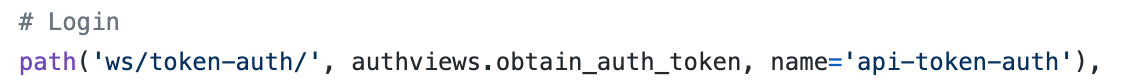
\includegraphics[width=\textwidth]{images/authtoken.png}
        \caption{URL da autenticação}
\end{figure}

\par A partir do momento do \textit{login}, o \textit{token} é guardado no \textit{front-end} e todos os pedidos à \textit{API} que necessitem de autorização são acompanhados deste mesmo \textit{token}. Assim, é garantida a autenticidade do utilizador ao fazer os pedidos.

\subsection{Autorização}

\par Mesmo depois do cliente efetuar o login, este não tem acesso a todas as informações. Para isso, criou-se uma função que verifica se o pedido é permitido. Por exemplo, um cliente só deverá ter acesso às suas compras, e não às compras dos restantes clientes. Assim, em cada pedido à \textit{API}, é verificado se o cliente que fez o pedido é o correto para a informação que é pedida. 

\begin{figure}[!h]
        \centering
        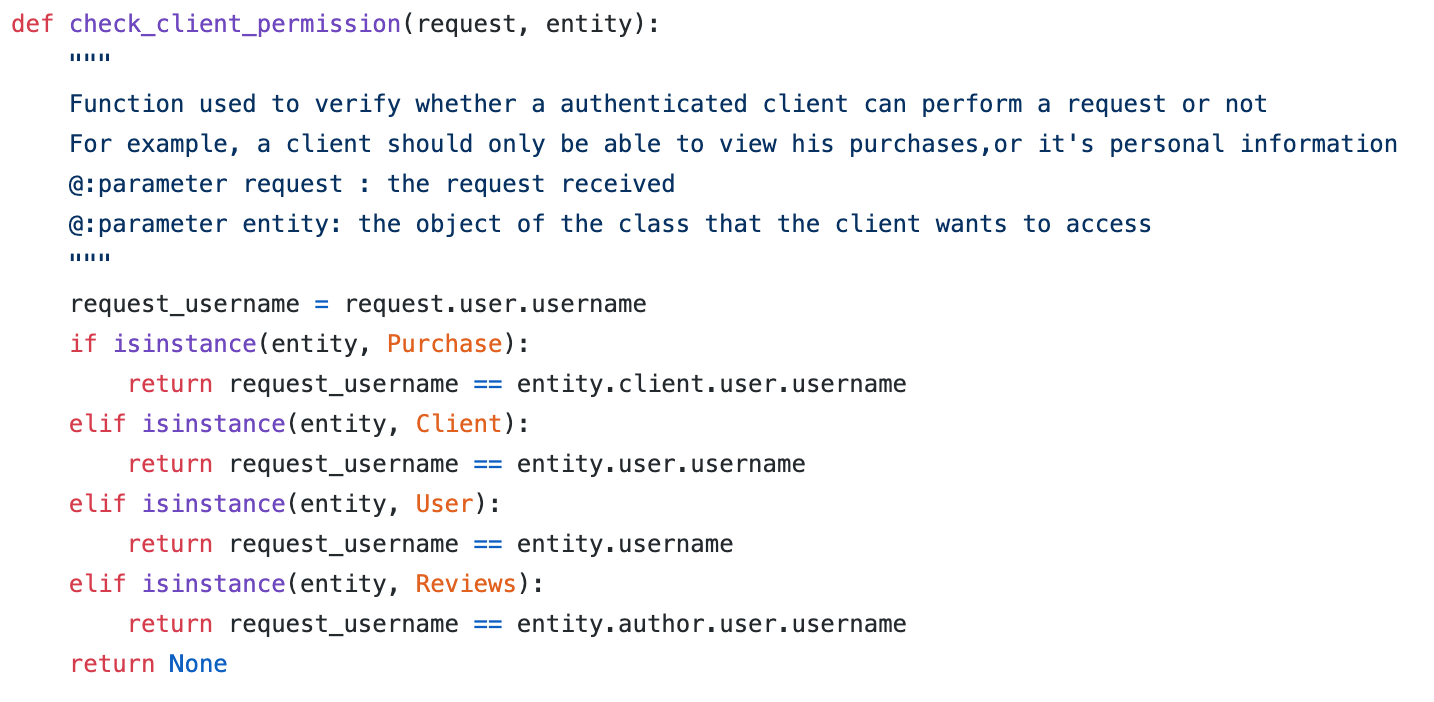
\includegraphics[width=400]{images/clientverif.png}
        \caption{Função de verificação das permissões}
\end{figure}

\newpage

\subsection{\textit{Views}}

\par As \textit{views} têm um papel importante na \textit{API}, visto que é nelas que estão presentes todos os pedidos disponíveis. Estão disponíveis os métodos \textit{GET}, \textit{PUT}, \textit{POST} e \textit{DELETE}. Cada \textit{endpoint}, nos \textit{URLs}, chama uma \textit{view} que define o método, as autorizações e só depois efetua o pedido, caso sejam validadas todas as condições.

\begin{figure}[!h]
        \centering
        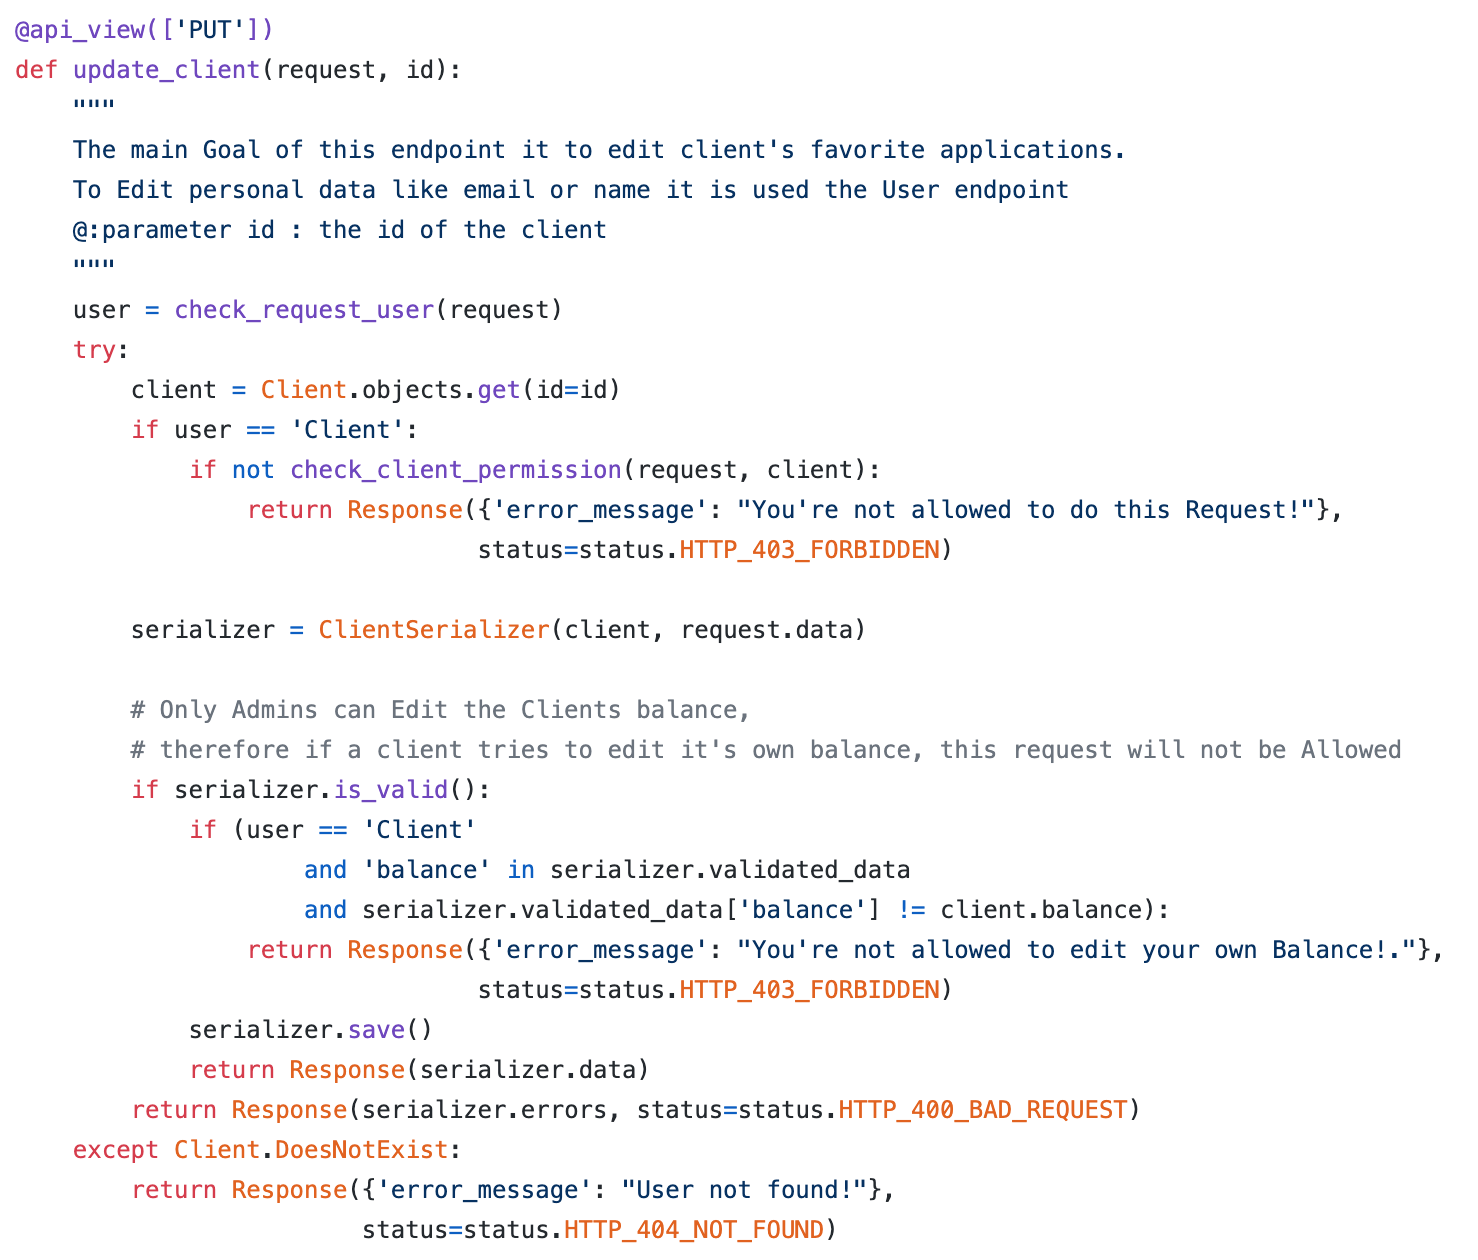
\includegraphics[width=\textwidth]{images/clientupdate.png}
        \caption{Exemplo de uma \textit{view} para o \textit{update (PUT)} das informações do cliente}
\end{figure}

\newpage

\subsection{\textit{Serializers}}

\par Toda a informação é processada pelos \textit{serializers}, utilizando o módulo \textit{'serializers.ModelSerializer'} importado do \textit{Django Rest Framework}. Estes permitem fazer verificações, tratar da informação e definir os campos a retornar e em que formato. Por exemplo, para o administrador criar um produto, basta fazer a seguinte chamada na \textit{view}:

\begin{figure}[!h]
        \centering
        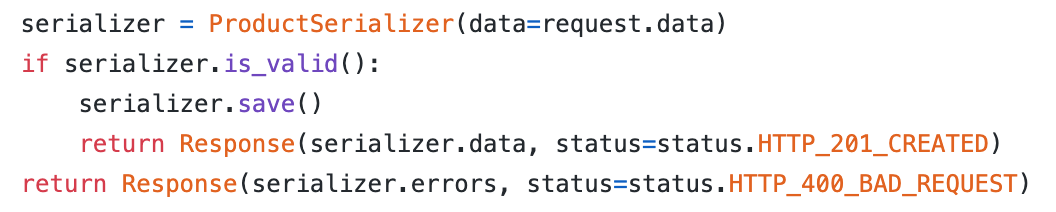
\includegraphics[width=\textwidth]{images/create_product.png}
        \caption{Chamada do \textit{serializer} do \textit{administrador}}
\end{figure}


\par O \textit{Serializer} vai se certificar que os campos introduzidos estão válidos e, em caso afirmativo, cria o produto, retornando a própria instância do produto: 

\begin{figure}[!h]
        \centering
        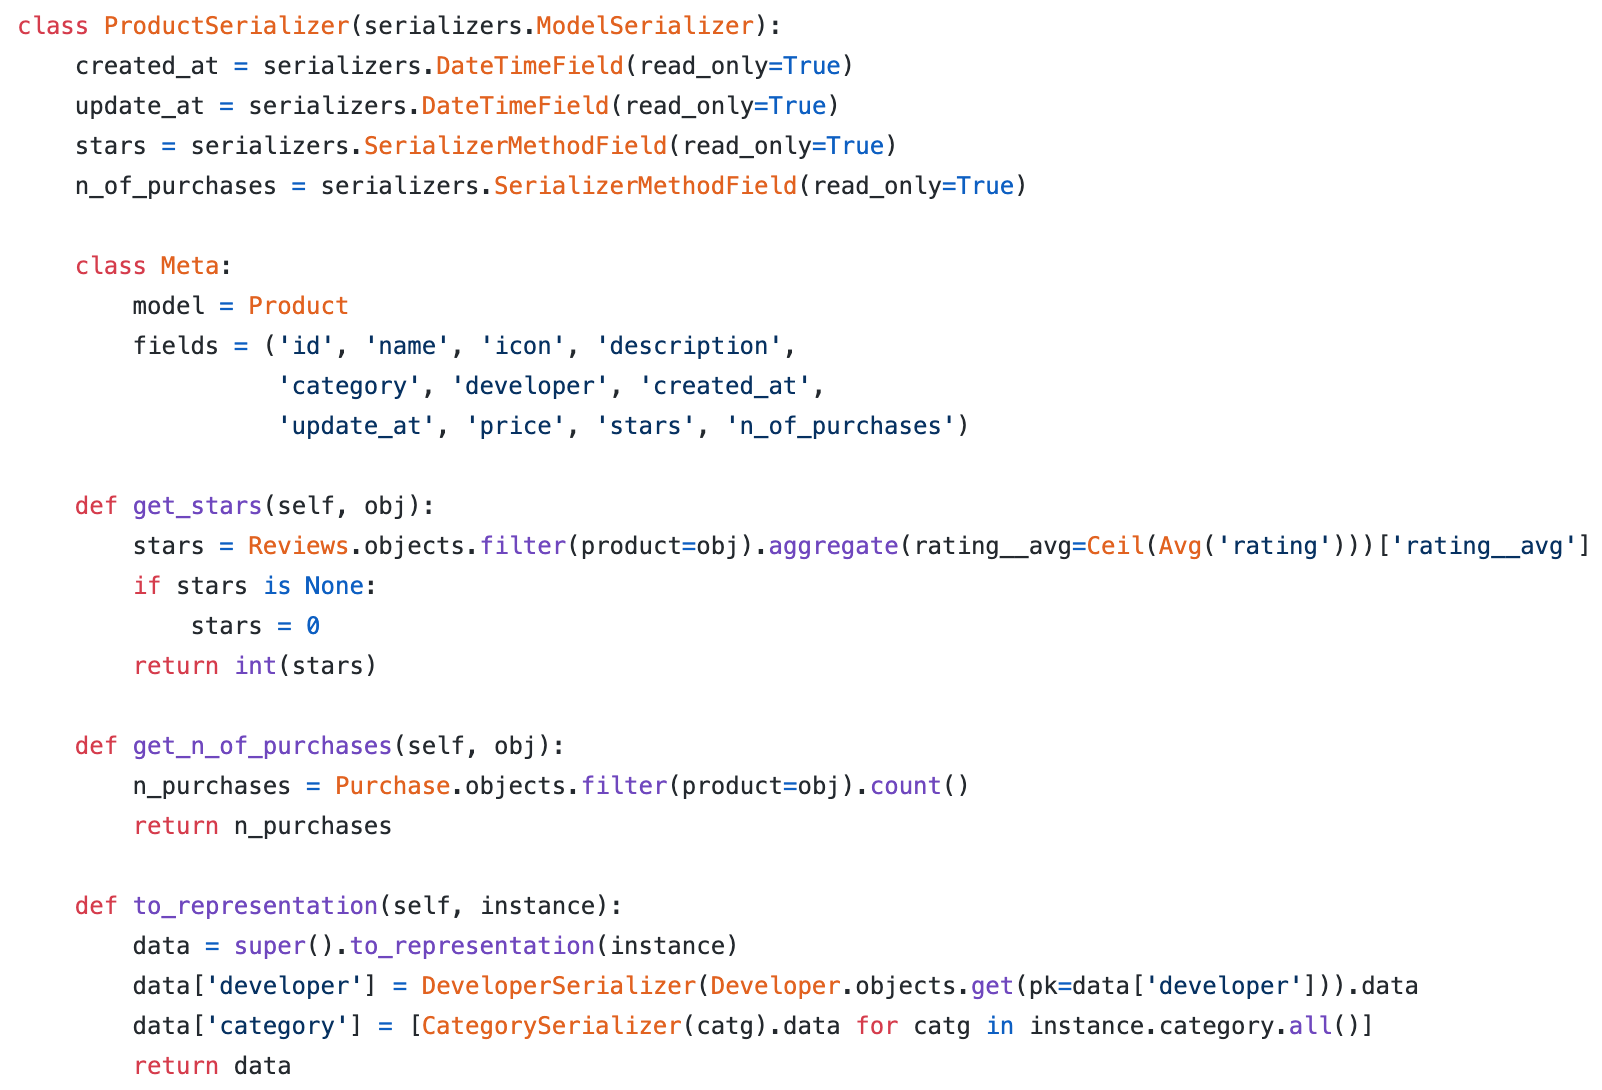
\includegraphics[width=\textwidth]{images/serializer.png}
        \caption{\textit{Serializer} do produto}
\end{figure}


\subsection{Documentação da \textit{API}}
\par Foi decidido, também, incluir um ponto importante em todas as \textit{REST APIs} que é a sua documentação. Para tal utilizou-se o módulo \textit{\textbf{drf-yasg}} do \textit{Python}. Este permite facilmente a criação de um \textit{endpoint} específico, e auto-gerado, contendo a listagem de  todos os métodos permitidos para cada \textit{endpoint} na nossa \textit{REST API} e também informação relativa à autenticação e autorização necessária para aceder a estes.

\begin{figure}[!h]
        \centering
        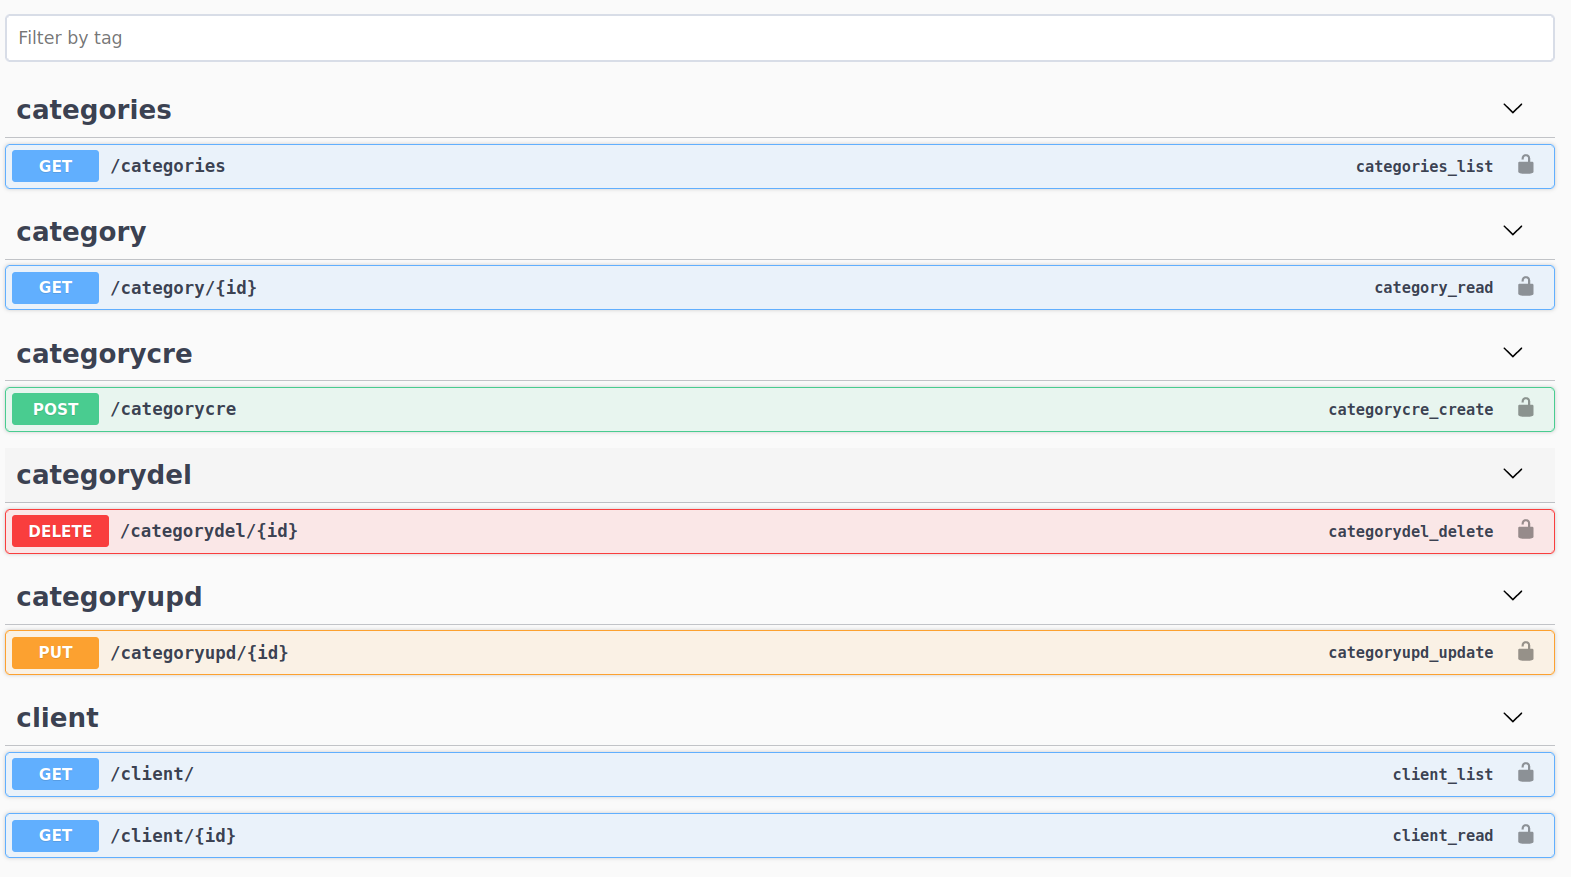
\includegraphics[width=\textwidth]{images/swagger.png}
        \caption{Excerto do conteúdo apresentado na página da documentação da \textit{API}}
\end{figure}


\clearpage
\section{Angular}
\par Todo o \textit{front-end} da nossa aplicação foi feito utilizando a Tecnologia \textit{Angular}. Esta \textit{framework} apresenta um Arquitetura \textit{Component-Based} e utiliza a linguagem \textit{TypeScript}, aproveitando-se as seguintes funcionalidades:
\begin{itemize}
  \item \textbf{Components}: Utilizou-se \textit{Components} para todas as \textit{views} e lógica proveniente, tentando a divisão ao máximo destes em \textit{"Sub-Components"}, de forma passar informação entre componentes dinamicamente;
  \item \textbf{Data Binding}: Com vista a mostrar os dados persistentes; 
  \item \textbf{Directives}: Com o intuito de manipular os elementos do DOM, com o comportamento adicional que se pretendia;
  \item \textbf{Services}: Usou-se serviços para obter todos os dados vindo da\textit{ REST API};
  \item \textbf{Routing}: Para a navegação dentro da interface;
  \item \textbf{Observables}: De forma a conseguir trabalhar com programação assíncrona;


\end{itemize}
    
\subsection{Apresentação de dados}

\par Para popular principalmente os \textit{forms} com dados, utilizou-se o \textit{Two-way Binding}, permitindo através da diretiva \textit{ngModel} a mudança de dados automática entre o modelo de dados e a \textit{view}, combinando a utilização de \textit{Property-Binding} com \textit{Event-Binding}.


\begin{figure}[!h]
        \centering
        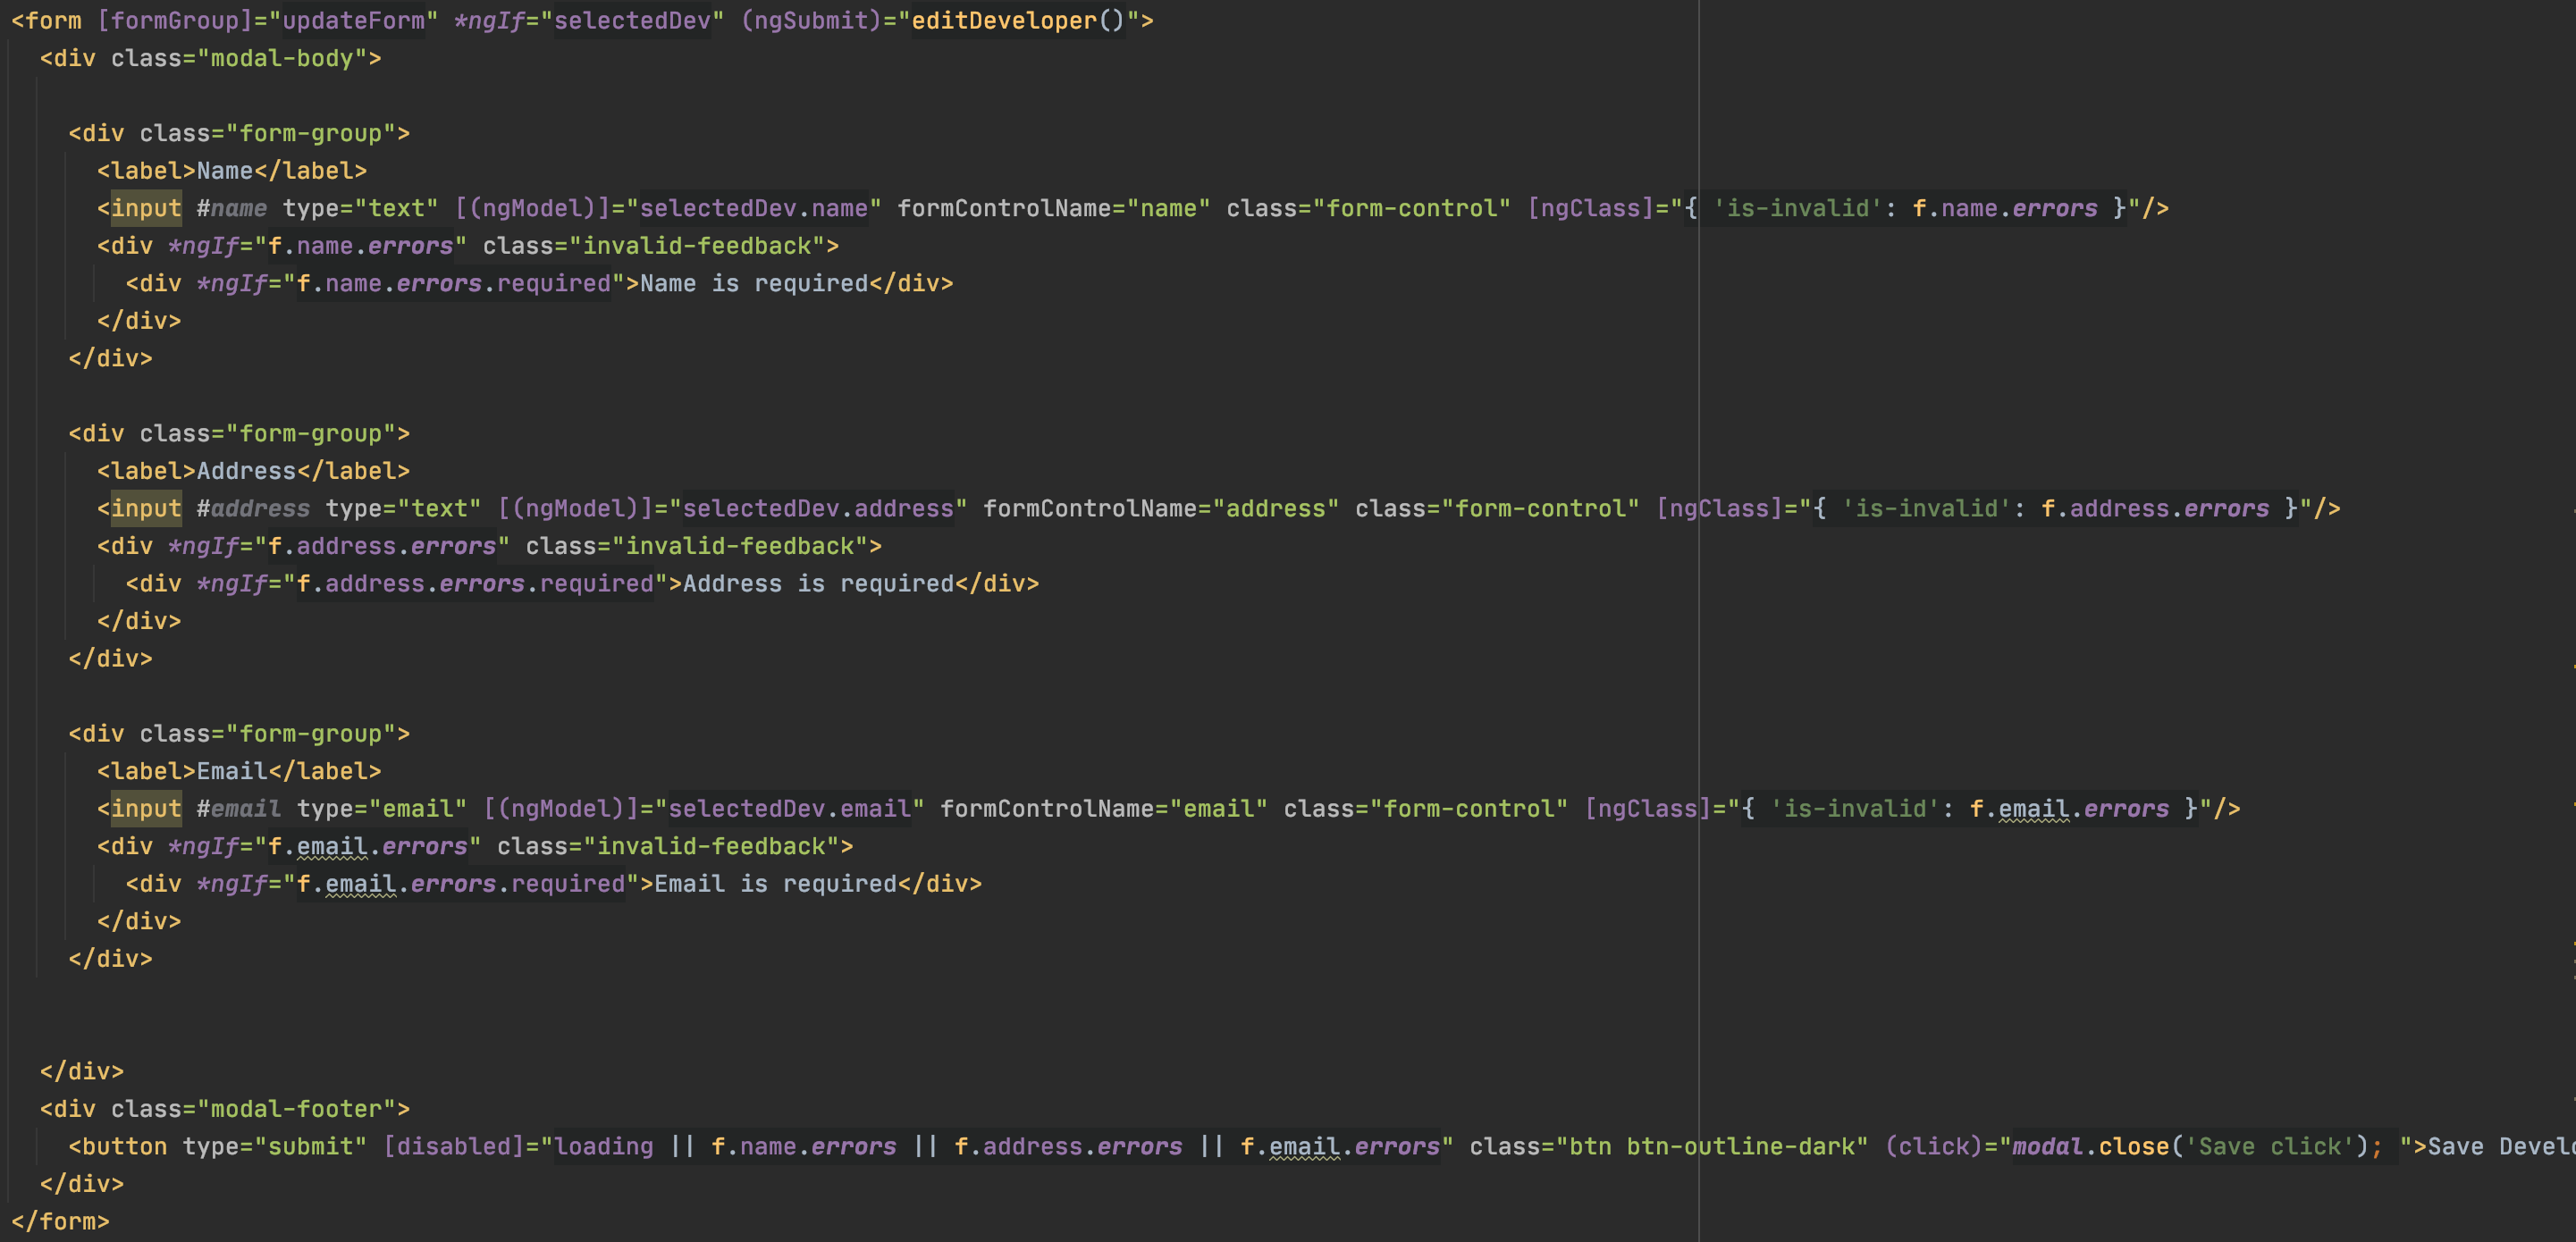
\includegraphics[width=\textwidth]{images/edit_dev.png}
        \caption{Exemplo da utilização de \textit{Two-way Binding}}
\end{figure}

\clearpage
\par Ao introduzir dados nas páginas gerais utilizou-se principalmente a \textit{Interpolation}, permitindo que uma variável do \textit{Angular} apareça com as suas informações na página.


\begin{figure}[!h]
        \centering
        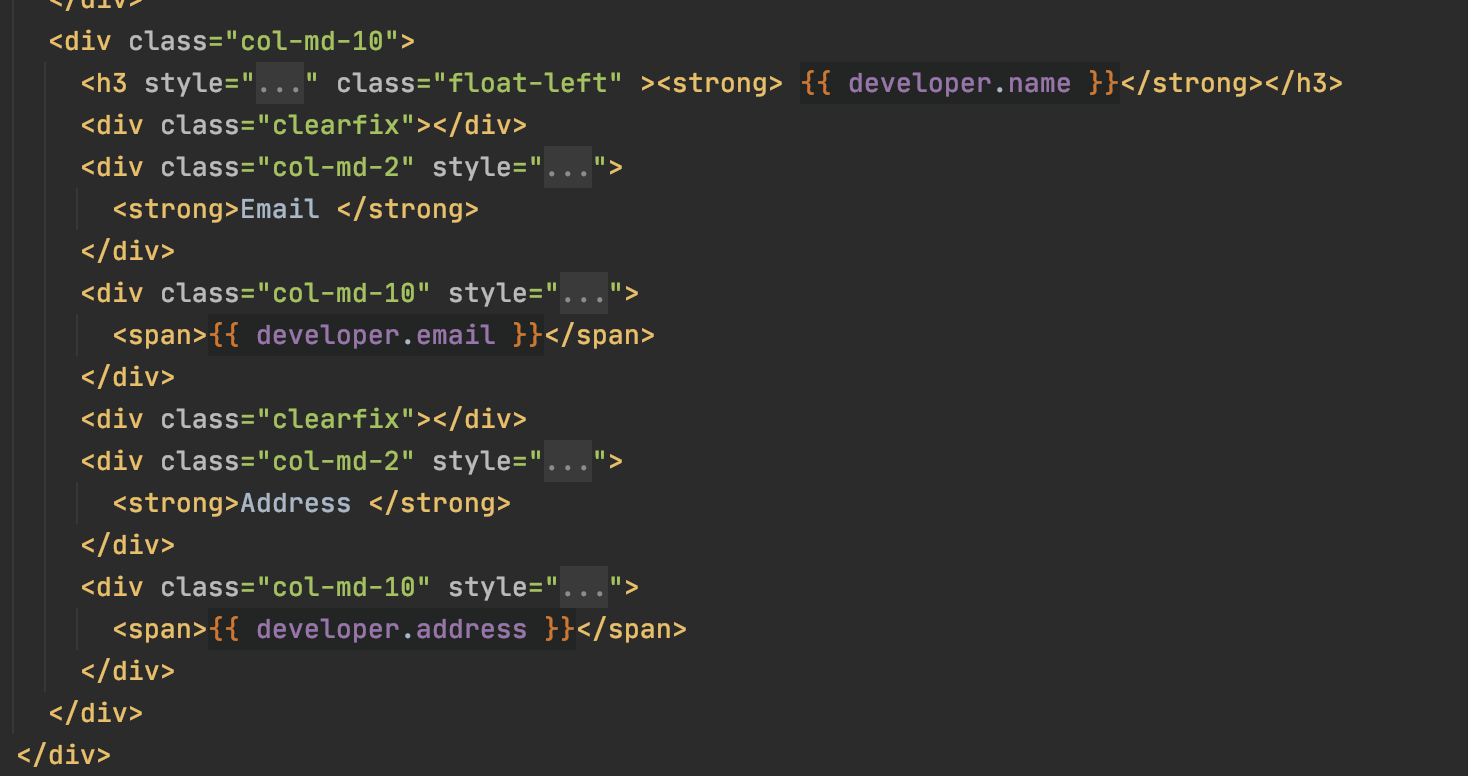
\includegraphics[width=\textwidth]{images/show_dev.png}
        \caption{Exemplo da utilização de \textit{Interpolation}}
        
\end{figure}

\clearpage

\par Como forma de aproveitar os dados fornecidos pelos \textit{WebServices} da \textit{DRF}, tentou-se procurar uma solução para conseguir passar informação entre \textit{Parent} e\textit{Child Components}. A solução encontrada foi a utilização dos Decoradores \textit{@Input()} e \textit{@Output()} aliados a \textit{Property} e \textit{Event Bindings}, o que facilmente permite o fluxo de dados, tal como é representado na imagem a seguir:
\begin{figure}[!h]
        \centering
        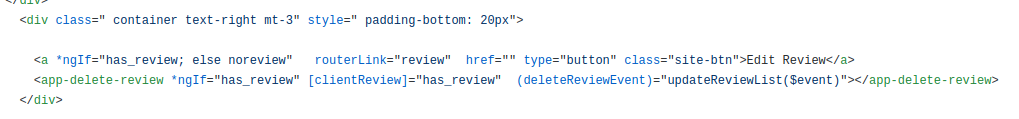
\includegraphics[width=\textwidth]{images/parent-child.png}
        \caption{Fluxo de Informação entre Parent e Child Components}
\end{figure}

\clearpage

\subsection{Serviços}
Como já foi referido,  utilizou-se Serviços para a obtenção dos dados que são disponibilizados pela \textit{REST API}, através de chamadas à mesma. De notar que, para a obtenção deste dados, todos os pedidos \textit{HTTP} são intersectados por um \textit{interceptor}, que tem o papel de introduzir o \textit{token} de autenticação nos \textit{headers} destes pedidos. Após isto acontecer o pedido segue naturalmente para a \textit{API}. 

\subsubsection{Obtenção de dados}
Na imagem seguinte, é possiver ver um exemplo de como se implementou os \textit{Services} do \textit{Angular}. Como é possível observar, a utilização destes é combinado com o uso de \textit{Observables}, permitindo a um componente dizer que quer uma informação sobre um objeto e só recolhe os dados quando estes chegarem, através de uma arquitetura \textit{Publish-Subscribe}. Além disto, é também utilizada \textit{Dependency Injection} de forma a que, quando este serviço for utilizado por \textit{components} que necessitem de dados da \textit{API}, o serviço seja injetado nesses \textit{components}. Assim, é permitida a reutilização de \textit{components} e impedir o uso de dependências \textit{hard-coded}.
\begin{figure}[!h]
        \centering
        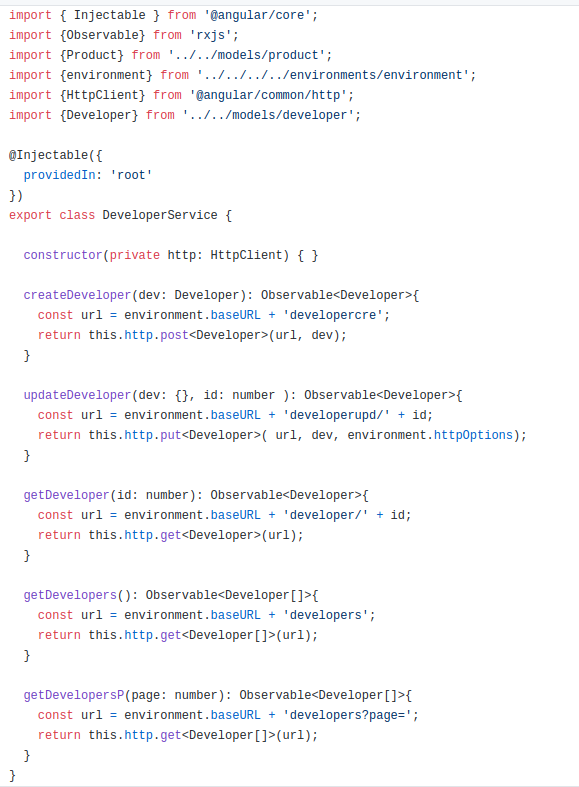
\includegraphics[width=275]{images/service1.png}
        \caption{Implementação de um Serviço}
\end{figure}
\clearpage
\subsubsection{Sistema de avisos}

\par É importante salientar neste documento um serviço específico utilizado, o \textit{Shared Service} (assim denominado por nós), que é um serviço que acaba por ser utilizado em muitos dos componentes. Neste serviço são implementados vários métodos que permitem a subscrição de eventos e o envio de eventos para os componentes que o subscreveram. Assim, foi permitido mostrar mensagens de Sucesso e Erro, através da utilização do componente \textit{AlertComponent} como subscritor de eventos de alertas, permitindo a reutilização de código para \textit{Feedback} ao utilizador final. 

\begin{figure}[!h]
        \centering
        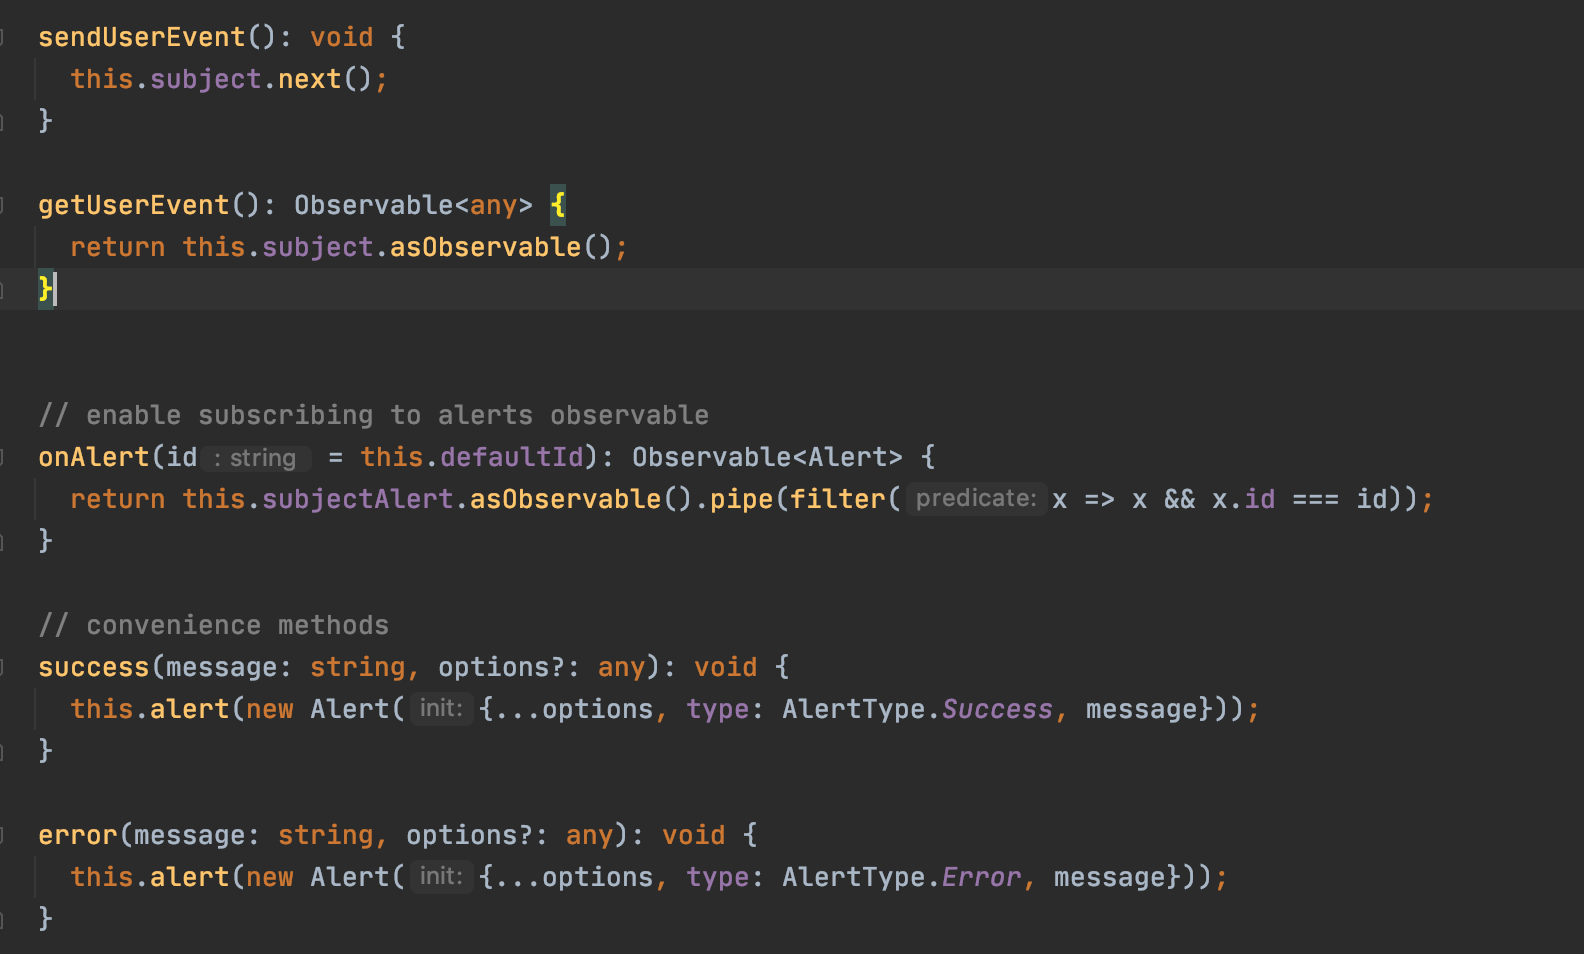
\includegraphics[width=300]{images/service_shared.png}
        \caption{Implementação do \textit{Shared Service} }
\end{figure}


\par Este serviço foi também utilizado para evitar que seja possível o utilizador estar a visualizar uma página à qual não tem acesso, por exemplo, caso o \textit{admin} esteja na página de administrador e este faça \textit{logout} através da \textit{navbar}, o componente desta envia um evento para avisar os componentes da página de administrador que o utilizador em questão já não permissão de visualização, existindo um redireccionamento.

\begin{figure}[!h]
        \centering
        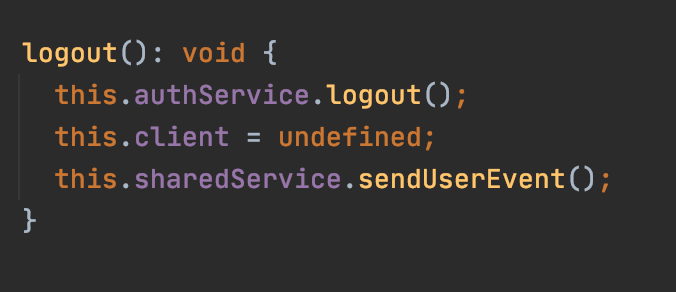
\includegraphics[width=300]{images/logout.png}
        \caption{Função de \textit{logout} do componente da \textit{navbar} que envia um evento para os componentes verificarem a sessão}
\end{figure}


\section{Execução do sistema}

\subsection{Localmente}

\par Para executar o serviço localmente é necessário executar tanto a aplicação \textit{web} como o serviço \textit{REST}.

\par Começando pela aplicação \textit{web} em \textit{Angular}, é necessário instalar as dependências deste projeto, executando \textit{\textbf{npm install}} na raiz do mesmo.

\par No caso do serviço \textit{REST} em \textit{Django}, é necessário instalar os \textit{\textbf{requirements}} que se encontram no ficheiro \textit{\textbf{requirements.txt}} na raiz deste projeto.

\par Feito isto, basta executar ambos os projetos através da linha de comandos ou de um \textit{IDE}.


\subsection{\textit{Deploy}}

\par Como especificado pelo professor, o \textit{deploy} foi realizado através das plataformas \textit{Heroku} e \textit{Python Anywhere} para a aplicação \textit{web} em \textit{Angular} e para o serviço \textit{REST} em \textit{Django REST Framework}, respetivamente.

\par O acesso ao sistema pode ser feito através dos seguintes endereços, contudo é importante referir que a ligação aos \textit{websites} terá de ser feita \textbf{apenas} por HTTP:

\begin{itemize}
    \item \textbf{Aplicação \textit{Web}} - \url{http://app-store-frontend.herokuapp.com}
    \item \textbf{\textit{REST API}} - \url{http://hugofpaiva.pythonanywhere.com}
    \item \textbf{Documentação da \textit{REST API}} - \url{http://hugofpaiva.pythonanywhere.com/swagger}
\end{itemize}

\subsection{Utilizadores}

\par Em ambos os cenários de execução podem ser usados estes utilizadores:

\hfill

\textbf{Administrador}
\begin{itemize}
    \item \textbf{username}: admin
    \item \textbf{password}: admin
\end{itemize}

\textbf{Clientes}
\begin{itemize}
    \item \textbf{username}: user1,user2,...,user10
    \item \textbf{password}: admin111
\end{itemize}

\clearpage

\section{Conclusão}

\par Para terminar, pensa-se que, de acordo com as metas estabelecidas pelo docente, o trabalho foi bem sucedido. Foram aprofundados conceitos relativos às tecnologias \textit{Angular} e \textit{Django Rest Framework} que sem dúvida será uma mais valia para o futuro profissional dos membros do grupo.
\par Alem disso, em termos de trabalho, foi criado um bom ambiente de equipa e uma boa gestão de \textit{backlog} que permitiu alcançar os objetivos de uma forma mais rápida e estável. 

\end{document}

